% begin module limit-at-infinity-ex3
\begin{frame}
\begin{example}[Example 3, p. 233]
\begin{columns}[c]
\column{.45\textwidth}
Evaluate $\lim_{x\to \infty} \frac{3x^2-x-2}{5x^2+4x+1}$.

\ \only<handout:0| -20>{%
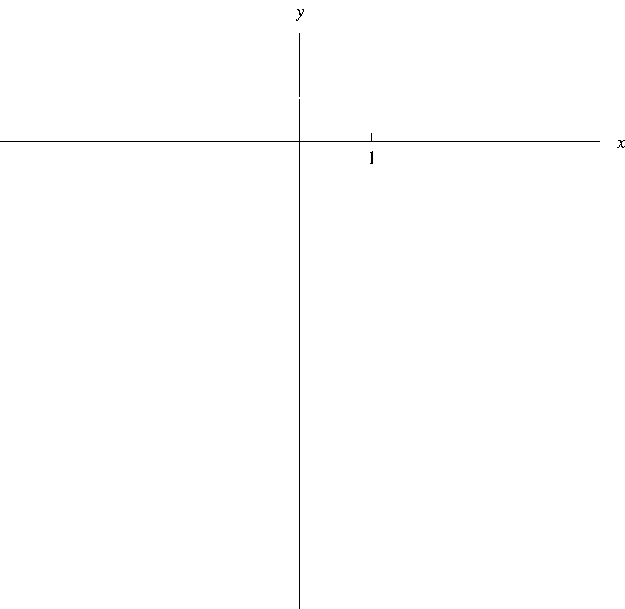
\includegraphics[width=5cm]{curve-sketching/pictures/04-04-ex3a.pdf}%
}%
\only<handout:0| 21-22>{%
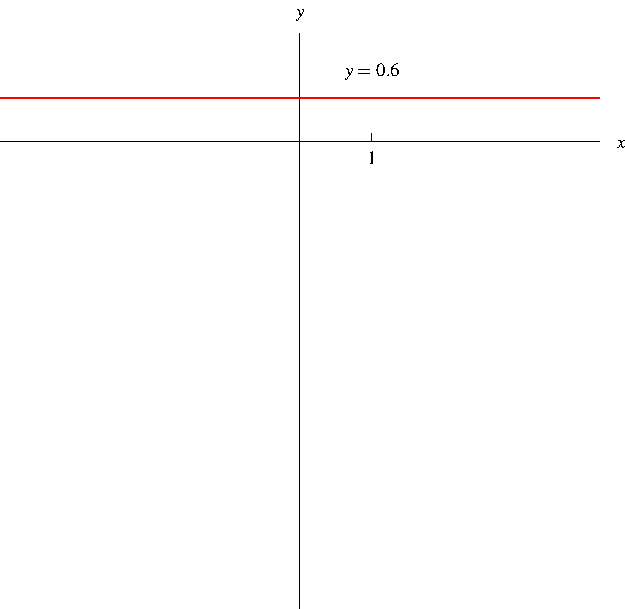
\includegraphics[width=5cm]{curve-sketching/pictures/04-04-ex3b.pdf}%
}%
\only<23->{%
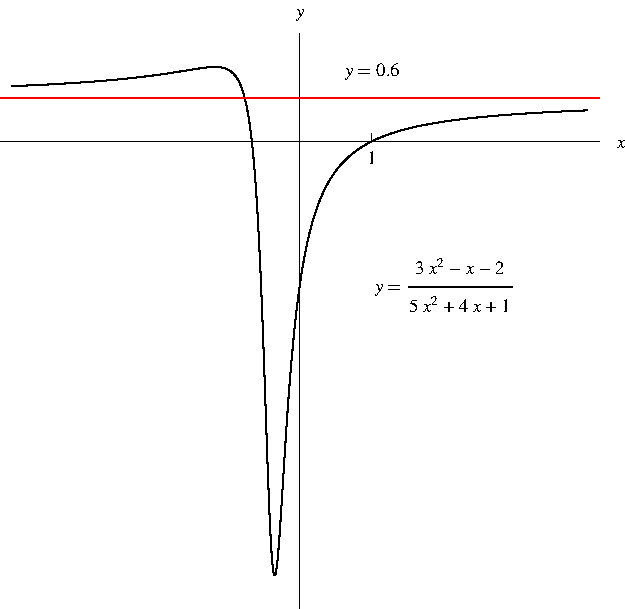
\includegraphics[width=5cm]{curve-sketching/pictures/04-04-ex3c.pdf}%
}%
\begin{itemize}
\item<22->  A similar calculation shows that the limit as $x\to -\infty$ is also $\frac{3}{5}$.
\end{itemize}
\column{.55\textwidth}
\begin{itemize}
\item<2-| alert@2-3>  Standard approach: divide top and bottom by the highest power of $x$ in the denominator.
\end{itemize}
\abovedisplayskip=0pt
\belowdisplayskip=0pt
\begin{eqnarray*}
&&%
\lim_{x\to \infty} \frac{\alert<handout:0| 4-5>{3x^2-x-2}}{\alert<handout:0| 6-7>{5\alert<handout:0| 3>{x^2}+4x+1}}\uncover<3->{\alert<handout:0| 3>{\cdot \frac{\alert<handout:0| 4-5>{\frac{1}{x^2}}}{\alert<handout:0| 6-7>{\frac{1}{x^2}}}}}%
\\%
& \uncover<4->{ = } &%
\uncover<4->{%
\lim_{x\to \infty} \frac{\uncover<5->{\alert<handout:0| 5>{3 - \frac{1}{x} - \frac{2}{x^2}}}}{\uncover<7->{\alert<handout:0| 7>{5+\frac{4}{x} + \frac{1}{x^2}}}}%
}%
\\%
& \uncover<8->{ = } &%
\uncover<8->{%
\frac{\displaystyle \alert<handout:0| 9-10>{\lim_{x\to\infty}3} - \alert<handout:0| 11-12>{\lim_{x\to\infty}\frac{1}{x}} - \alert<handout:0| 13-14>{2\lim_{x\to\infty}\frac{1}{x^2}}}{\displaystyle \alert<handout:0| 15-16>{\lim_{x\to\infty}5} + \alert<handout:0| 17-18>{4\lim_{x\to\infty}\frac{1}{x}} + \alert<handout:0| 19-20>{\lim_{x\to\infty}\frac{1}{x^2}}}%
}%
\\%
& \uncover<9->{ = } &%
\uncover<9->{%
\frac{\uncover<10->{\alert<handout:0| 10>{3}} - \uncover<12->{\alert<handout:0| 12>{0}} - \uncover<14->{\alert<handout:0| 14>{0}}}{\uncover<16->{\alert<handout:0| 16>{5}} + \uncover<18->{\alert<handout:0| 18>{0}} + \uncover<20->{\alert<handout:0| 20>{0}}}%
}%
\uncover<21->{ = } %
\uncover<21->{%
\frac{3}{5}%
}%
\end{eqnarray*}
\end{columns}
\end{example}
\end{frame}
% end module limit-at-infinity-ex3
